\documentclass{article}
\usepackage{
  amsmath, amsthm, amssymb, amsfonts,
  mathtools, xfrac, dsfont, mathrsfs, bm
  }
\usepackage{hyperref, float, parskip}
\usepackage[margin=0.8in]{geometry}
\usepackage[justification=centering,labelfont=bf]{caption}
\renewcommand{\arraystretch}{1.3}

% grouping and bookending
\newcommand{\pr}[1]{\left(#1\right)}
\newcommand{\br}[1]{\left[#1\right]}
\newcommand{\cbr}[1]{\left\{#1\right\}}
\newcommand{\floor}[1]{\left\lfloor#1\right\rfloor}
\newcommand{\ceil}[1]{\left\lceil#1\right\rceil}
\newcommand{\abs}[1]{\left|#1\right|}
\newcommand{\norm}[1]{\left\lVert#1\right\rVert}
\newcommand{\ip}[1]{\left\langle#1\right\rangle}
\renewcommand{\vec}[1]{\left\langle#1\right\rangle}
% derivatives
\newcommand{\der}[2]{\frac{d #1}{d #2}}
\newcommand{\mder}[2]{\frac{D #1}{D #2}}
\newcommand{\pder}[2]{\frac{\partial #1}{\partial #2}}
% common bold and script letters
\newcommand{\C}{\mathbb{C}}
\newcommand{\E}{\mathbb{E}}
\newcommand{\F}{\mathcal{F}}
\newcommand{\G}{\mathcal{G}}
\renewcommand{\L}{\mathscr{L}}
\newcommand{\N}{\mathbb{N}}
\renewcommand{\O}{\mathcal{O}}
\renewcommand{\P}{\mathbb{P}}
\newcommand{\Q}{\mathbb{Q}}
\newcommand{\R}{\mathbb{R}}
\renewcommand{\S}{\mathbb{S}}
\newcommand{\Z}{\mathbb{Z}}
% math operators
\DeclareMathOperator{\Cov}{Cov}
\DeclareMathOperator{\Var}{Var}
\let\Re\relax
\DeclareMathOperator{\Re}{Re}
\let\Im\relax
\DeclareMathOperator{\Im}{Im}
\DeclareMathOperator{\diag}{diag}
\DeclareMathOperator{\tr}{tr}
\DeclareMathOperator*{\argmax}{arg\,max}
\DeclareMathOperator*{\argmin}{arg\,min}
% misc
\newcommand{\mat}[1]{\begin{bmatrix}#1\end{bmatrix}}
\newcommand{\ind}[1]{\mathds{1}_{#1}}
\renewcommand{\epsilon}{\varepsilon}

\newcommand {\beq} {\begin{equation}}
\newcommand {\eeq} {\end{equation}}

\setlength\parindent{0pt}

%\title{High Performance Computing: Final Project Report}
%\author{Paul Beckman, Mariya Savinov}
\begin{document}

\begin{center}
{\bf
High Performance Computing: Final Project Report \\
}
Paul Beckman, Mariya Savinov\\
Repo location: \url{https://github.com/pbeckman/fast-summation/}
\end{center}

%\maketitle

\section{Introduction}
Many settings in physics involve a collection of particles/masses interacting through conservative forces (forces which can be defined by some scalar potential function $u$), for example the electrostatic potential for a collection of point charges, or the gravitational potential for a collection of masses. In order to determine the particle dynamics, one must evaluate the total system potential at each particle point. As such, particularly when there are a large number $N$-many particles, we are interested in the rapid evaluation of this potential.

Let us consider points $x_1,...,x_n\in[0,1]=I$ with charges $q_1,...,q_n$ (equivalently, masses). We limit the positions to a one-dimensional problem to focus on the computational aspects, but imagine these particles to be embedded in $\R^3$ so that the potential at $x$ due to a particle at point $x_j$ with unit charge is
\beq
        \phi(x) = \frac{C}{\abs{x-x_j}}.
\eeq
where $C$ is some scaling factor (e.g. the Coulomb constant) taken in our calculations to be $C=1$. The total potential is then
\beq
        u(x_i) = \sum_{j=1}^n q_j \phi(\abs{x_i - x_j}) = \sum_{j=1}^n \dfrac{q_j}{\abs{x_i-x_j}}
\label{eq:potential}
\eeq
which we seek to evaluate for each $x_i$. The idea will be to hierarchically partition the interval and take advantage of Taylor series expansions to approximate far-field contributions as given by a single particle at the center of mass.

\section{Barnes-Hut Tree Code}
In order to reduce the cost of $\O(n^2)$ direct summation, Barnes and Hut \cite{barnes1986hierarchical} proposed a method that approximates the potential induced by faraway points by considering only the centers of mass of distant groups of points. This is essentially a zeroth order version of the multipole method we present here, which is itself a simplification of the fast multipole method \cite{greengard1987fast}.

The basic concept of the multipole tree-code we study here (adapted from Long Chen's FMM notes \cite{chenintroduction}) is to consider a point $y$ and Taylor expand $\phi(x_j - y)$ for collections of points $x_j$ around a \textit{center of mass} $x_*$ for which the ratio
\begin{equation}
  \delta = \frac{x_j-x^*}{x^*-y}
\end{equation}
is small. This results in the following expansion
\begin{align}
  \phi(x_j-y)
  &= \phi(x^*-y)\phi(1+\delta)\\
  & \approx \phi(x^*-y)\br{\sum_{m=0}^p \dfrac{\phi^{(m)}(1)}{m!}\delta^m + O(\delta^{p+1})}\\
  & = \sum_{m=0}^p a_m(x_j-x^*)S_m(x^*-y) + O(\delta^{p+1})
\end{align}
crucially this expansion is order $p$ in $\delta$, and thus we can obtain arbitrarily high accuracy by computing higher-order terms in the Taylor expansion.

Take $\delta = \frac{1}{2}$. Then we consider points $x_j$ for which $\frac{x_j-x^*}{x^*-y} < \frac{1}{2}$ to be the \textit{far-field} of $y$. For such points, the potential contribution can be approximated by
\begin{equation}
  \sum_{j\in\text{far-field}} q_j\phi(x_j-y) \approx \sum_{m=0}^p \underbrace{\br{\sum_{j\in\text{far-field}} q_j a_m(x_j-x^*)}}_{\text{weight }w} S_m(x^*-y)+ O(\delta^{p+1})
\end{equation}
In order evaluate the far-field at multiple levels, the key idea is to compute terms involving only far-field cells \emph{not included at higher levels}. This is the so-called \textit{interaction list} shown in Figure \ref{fig:interaction}. For a point $y$, the potential is therefore approximated by
\begin{equation}
  u(y) = \sum_{\ell=1}^{O(\log N)}\sum_{m=0}^p w_{\ell,k(\ell),m} S_m\pr{x_{\ell, k(\ell)}^* - y} + O\pr{\frac{1}{2^p}}.
\end{equation}
The multipole Barnes-Hut algorithm thus consists of two steps. The first step is to compute the weight $w_{l, k, m}$ for box at each level which results in a total cost of $\O(n\log n)$. The second step is to sum the weights in each interaction list at each level, which contributes only $\O(n)$ work. Thus the overall complexity is $\O(n\log n)$, which is confirmed by our serial implementation (see Figure \ref{fig:scaling}).

\begin{figure}
  \centering
  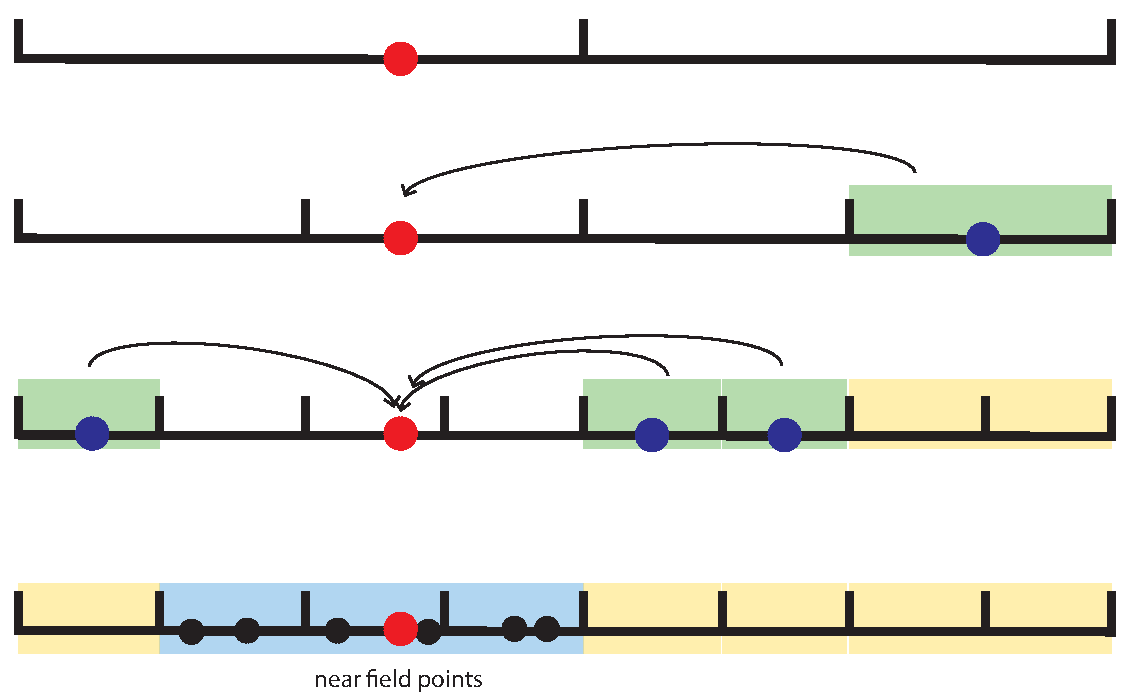
\includegraphics[width=0.55\textwidth]{./figures/interaction_list.pdf}
  \caption{Interaction list (green), uncomputed far-field (yellow), and near-field computed at the finest level (blue) for a four level tree.}
  \label{fig:interaction}
\end{figure}

\begin{figure}
  \centering
  \includegraphics[width=0.55\textwidth]{./figures/varying_n_m32_p5.png}
  \caption{Confirmation of $\O(n\log n)$ scaling for varying $n$ with fixed number $p=5$ of multipole moments and fixed number 32 points in a box at the finest level.}
  \label{fig:scaling}
\end{figure}


\section{Parallelism}
We parallelize this tree-code with OpenMP. Recall that this {\tt barnes\_hut} algorithm runs in two steps: first the weights are computed via {\tt compute\_weights} and then the potential is computed using the pre-computed weights by {\tt compute\_potential}. In each step, starting from level 0 the tree is traversed by the function calling itself at each daughter cell. Within a cell, {\tt compute\_weights} includes work that loops over each moment and each point in the cell. Meanwhile, {\tt compute\_potential} has work split in two parts: adding near field terms, which involves loops over each point pair in the cell, and adding far field terms, which involves loops over each moment and each point in the cell. This structure suggests two options of parallelism.
\subsection{Loop parallelism}
The first option is to parallelize the loops involved in computing the weights, adding near-field terms, and adding far-field terms. In each cell for each of these loop sections, a parallel region is opened and the manager thread creates a team with the user-specified number of threads. Generally the work for each thread for a given loop is fairly similar, so the default static mapping is appropriate (and use of, for example, dynamic scheduling we see only serves to yield a slight {increase} in runtime).\\\\
However, the potential problem lies in the \emph{varying sizes} of these loops depending on location in the tree. At the finest level, there are few points in each cell (sometimes less than the number of threads), so there is little benefit to loop parallelism. We will see that, indeed, if the max points at the smallest level or total moment number $p$ are small, then there is a large overhead cost in including these parallel directives in small cells (as observed through the runtime).
\begin{figure}
  \centering
  \includegraphics[width=0.55\textwidth]{./figures/{tree_parallelism}.pdf}
  \caption{Tree traversal for 'Work parallelism' option.}
  \label{fig:tree_parallel}
\end{figure}
\subsection{Work parallelism}
The second option is to distribute the work in the tree evenly among available threads. The idea is that in both {\tt compute\_weights} and {\tt compute\_potential}, as long as there are are extra threads available, the recursive calls to the two daughter cells should be done by two independent threads. This can be done by utilizing the {\tt section} directive in OpenMP and {explicitly} enabling nesting, so that each recursive function call opens new threads which run side by side with other threads opened at the same level.\\\\
Suppose for example that there are 4 total available threads. The tree-traversal then occurs as shown in Fig.~\ref{fig:tree_parallel}, where each color represents a unique thread. At level zero, there is only the master thread (red), which then recruits another thread (blue) to handle the second daughter cell at level 1. Each of these threads (red and blue) at level 2 do the same by recruiting the purple and orange threads for the work at level 2. After this point, there are no available threads, so the remainder of the tree is evenly distributed\footnote{presuming uniform distribution of points} among these four threads which handle the work sequentially for their individual section. In the more general sense, if there are $r$ total threads, at each tree level $\ell<O(\log r)$ the recursive call for daughter cells should be distributed by OpenMP {\tt sections}.\\\\
The only potential problem lies in the use of nested parallelism, as it is unclear how much overhead or hidden work is involved in determining thread availability and using nested recursive {\tt section} directives. However, this is likely minimal as compared to the overhead we expect and ended up observing for the loop parallelism option.
\section{Results}
\subsection{Comparing Parallel Options}
\begin{figure}
  \centering
  \includegraphics[width=0.75\textwidth]{./figures/varying_m_n32768_p5_4_8.png}
  \caption{Comparison of two parallelism options against the serial implementation for two choices of thread number, varying the number of levels in the tree (i.e. the number of max points at the finest level) while keeping the number of points and largest moment $p$ fixed. Runtimes computed on crackle1 (Intel Xeon E5630, 2.53 GHz).}
  \label{fig:varying_m}
\end{figure}
The difference between the two parallelism options and their effectiveness are best initially compared by considering a fixed number of points $n=2^{15}$ with largest moment $p=5$ and varying the number of points in the smallest box (equivalently, varying the number of levels in the tree). Fig.~\ref{fig:varying_m} shows the runtimes for the Barnes-Hut algorithm when it is run in serial\footnote{OpenMP is not included during code compilation for this case} (black) and when it is run with loop parallelism (ver1, orange) and work parallelism (ver2, blue) for the cases of both 4 threads and 8 threads.\\\\
For the serial implementation, it makes sense that the runtime is shortest for few max points at the smallest level, as the approximation of the tree algorithm is taken advantage of best here. If there are many points at the smallest level of the tree, then there are more direct near-field particle-particle interactions to compute, so as expected you approach the cost of just direct calculation of the potential without any tree structure at all.\\\\
The primary difference between the two parallelisms becomes very clear in Fig.~\ref{fig:varying_m}. For loop parallelism (orange), when there are few points at the finest level, the overhead cost of parallelizing the short/small loops at the lower levels becomes significant, and the runtime greatly exceeds that of the serial code. However, speedup can still be achieved, if the max points in the smallest box is sufficiently large (so the tree has fewer levels). If one uses less threads, e.g. the dotted orange line as compared to the solid orange line, then it naturally becomes less expensive for small minimum box sizes as there are fewer threads to synchronize and manage for small loops.  However, the speedup observed on the right side of the figure is smaller if there are less available threads.\\\\
Unlike loop parallelism, work parallelism (blue) \emph{always performs better than the serial code} and is \emph{always faster with more threads}, as can be seen by the dotted line (4 threads) being consistently larger than the solid line (8 threads). It is clear, at least in regard to 'universal' speedup, that the second type of parallelism where work is evenly distributed among threads is the better choice. It remains to perform some scaling analysis, to determine how the speedup and efficiency of both parallelisms.

\subsection{Strong Scaling}
\begin{figure}
  \centering
  \includegraphics[width=0.48\textwidth]{./figures/strong_scalability.png} %
  \includegraphics[width=0.48\textwidth]{./figures/strong_scalability2.png}
  \caption{Results for the two parallelism options in the case of $n=32768$ points, $2048$ points in the smallest box, and $p=5$ moments. (Left) Algorithm runtime is plotted against thread number (from $2$ to $16$ threads). (Right) The speedup $S(r) = t(1)/t(r)$ where $t(1)$ is given by the runtime of the serial case (no parallelism) is plotted against thread number with the ideal speedup line shown. Loop parallelism is shown in orange, and work parallelism is shown in blue. Runtimes computed on crunchy1 (AMD Opteron 6272, 2.1 GHz).}
  \label{fig:strong_scaling}
\end{figure}
To test the strong scaling of the parallelism options, we test how the runtime changes as the number of threads/processors increases for a fixed case. We consider the case of $n=32768$ points, $2048$ points in the smallest box, and $p=5$ moments, since Fig.~\ref{fig:varying_m} showed that both parallelisms yield speedup in this case with more threads decreasing runtime.  The left plot of Fig.~\ref{fig:strong_scaling} confirms the expectations that as the number of threads increases, the runtime should decrease. It also once again indicates that the work parallelism (ver2, blue) is a better choice than loop parallelism (ver1, orange) as the runtimes are consistently smaller.\\\\
In order to determine how close to ideal speedup these parallelisms are, we consider the ratio of the serial runtime to the parallel runtime and ideally expect a linear increase with thread number (i.e., ideal speedup is $S(r) = t(1)/t(r) = r$ for $r$ threads). The right plot of Fig.~\ref{fig:strong_scaling} shows that the work parallelism yields closer to ideal speedup than loop parallelism, though both veer quite far from the ideal line (dotted, black) as the number of threads increases. For work parallelism, 16 threads yields a speedup that is about $\sim 10$ while for loop parallelism the speedup is only $\sim 5$. Once again, it is clear that work parallelism is the better of two parallelisms in this problem.

\subsection{Weak Scaling}
\begin{figure}
  \centering
  \includegraphics[width=0.48\textwidth]{./figures/weak_scalability.png} %
  \includegraphics[width=0.48\textwidth]{./figures/weak_scalability2.png}
  \caption{Results for the two parallelism options in the case of $n=8192r$ points for $r$ threads, $2048$ points in the smallest box, and $p=5$ moments. (Left) Algorithm runtime is plotted against thread number (from $2$ to $16$ threads), where problem size increases linearly with number of threads. (Right) The efficiency $t(1)/t(r)$, where $t(1)$ is given by the runtime of the serial code (no parallelism, $r=1$), is plotted against thread number $r$ with the ideal efficiency line shown. Loop parallelism is shown in orange, and work parallelism is shown in blue. Runtimes computed on crunchy1 (AMD Opteron 6272, 2.1 GHz).}
  \label{fig:weak_scaling}
\end{figure}
In addition to the strong scaling study above, we also performed a weak scaling study in which we increase the number of threads proportionally with $n$. We consider $n=8192r$ points using $r$ threads with 2048 points in the smallest box and $p=5$ moments.

Under perfect weak scaling one would observe a constant runtime in this setting. Between 2 and 4 threads, however, there is a significant slowdown in which the efficiency is reduced to approximately one half for both modes of parallelism. This trend does not continue strongly for work parallelism, and we see only a modest increase in cost as we expand to 16 threads. Loop parallelism suffers a more dramatic performance loss at this higher level of parallelism. See Figure \ref{fig:weak_scaling}. These tests indicate that work parallelism achieves superior performance even in the weak scaling setting where the loops are scaled proportionally with the problem size.

\section{Conclusion and Discussion}
In sum, we have successfully implemented the serial Barnes-Hut type tree-code and parallelized the algorithm in two ways -- loop parallelism and work parallelism. Through various testing, including strong and weak scaling, it is clear that work parallelism yields consistent, overall superior speedups as compared to loop parallelism. The overhead costs of including parallel directives for small/low work loops is significant; \emph{how} significant is somewhat machine dependent, but it is consistently worse than work parallelism when the tree has close to maximal levels.\\\\
The work parallelism implementation yields itself well to an extension of this project using MPI, where below level $O(\log(x))$ for $x$ cores the tree could be evenly distributed between cores and the work parallelism be implemented for each sub-tree at each core. The question would become how to minimize communication between cores, and what information is necessary to transfer at what points in time.

\bibliographystyle{plain}
\bibliography{refs}

\end{document}